\documentclass[10pt]{article}
\usepackage[top=1in, bottom=1.25in, left=1in, right=1in]{geometry}
\usepackage{amsmath}
\usepackage{amssymb}
\usepackage{enumitem}
\usepackage{graphicx}


\usepackage{fancyhdr}
\pagestyle{fancy}
\lhead{MATH7241: Project Report}
\rhead{David Zhao\\Benjamin Quiring\\\today}
\setlength{\headheight}{40pt}

\newcommand{\solution}{\textbf{Solution. }}
\newcommand{\deff}{\underline{Def. }}
\newcommand{\thm}{\underline{Theorem. }}
\newcommand{\lemma}{\underline{Lemma. }}
\newcommand{\corollary}{\underline{Corollary. }}
\newcommand{\proof}{\emph{Proof }}

%\newenvironment{proof}{\par\noindent{\it Proof.}\hspace*{1em}}{$\Box$\bigskip}

\setlength{\parindent}{0em}
\setlength{\parskip}{0.5em}
\begin{document}
\section{Data}
We downloaded a history of terminal commands for a UNIX computer from Perdue
University back in 1998. A sample of the data looked like:
\begin{verbatim}
cd
<1>
ll
vi
<1>
ll
emacs
\end{verbatim}

The data tracked 8 users' commands over a two year period. Since each user has
their own preference of UNIX terminal commands, we decided to only use data from
one user. We decided to only analyze one user because we were more interested in
the distribution of commands typed for a given user rather than looking for
trends among the commands typed by all users.

Where a \texttt{<\#>} represents the number of arguments given to a command.
This was done to preserve the user's privacy. We cleaned the data as follows:
\begin{itemize}
  \item We combined a command with the number of arguments passed with it. For
    example \texttt{cd<1>} is different from \texttt{cd} which is also different
    from \texttt{cd<2>}.
  \item We ignored operators like \texttt{; , -, |}, thus not considering them
    as commands. We also ignored any lines of text that weren't typed by the
    user.
\end{itemize}

After cleaning the data as described above, the resulting data consisted of one
UNIX terminal command per line. Because there were over $700$ unique commands,
we chose the $28$ most common occurring commands to be the states of our Markov
chain and proceeded to further filter the data by deleting commands that are not
the $28$ most common. From here we did the intuitive thing to consider filtered
data as a Markov chain where the initial state is the first command in the data
and at each timestep the chain moves from the current command to the command
just after it.

One issue with this representation is that many edges in the
chain are removed by our filtering. If, in the original dataset, there was a
sequence $Y \rightarrow X_1 \rightarrow ...  \rightarrow X_n \rightarrow Z$
where $Y$ and $Z$ are among the top $28$ commands, and $X_1,\dots, X_n$ are
commands not among the top $28$, then this reduced to $Y \rightarrow Z$. We
decided that this was the best way to filter the data because if we didn't add
an edge between $Y$ and $Z$, then the chain would have very strange fragments
(and the plot of the chain would not work). If we had instead chosen to
represent the chain with $700$ states the graphical representation of this chain
would be very hard to comprehend. Therefore we chose to represent our chain as
stated because the alternatives didn't seem any better.

\begin{figure}[!htb]
  \centering
  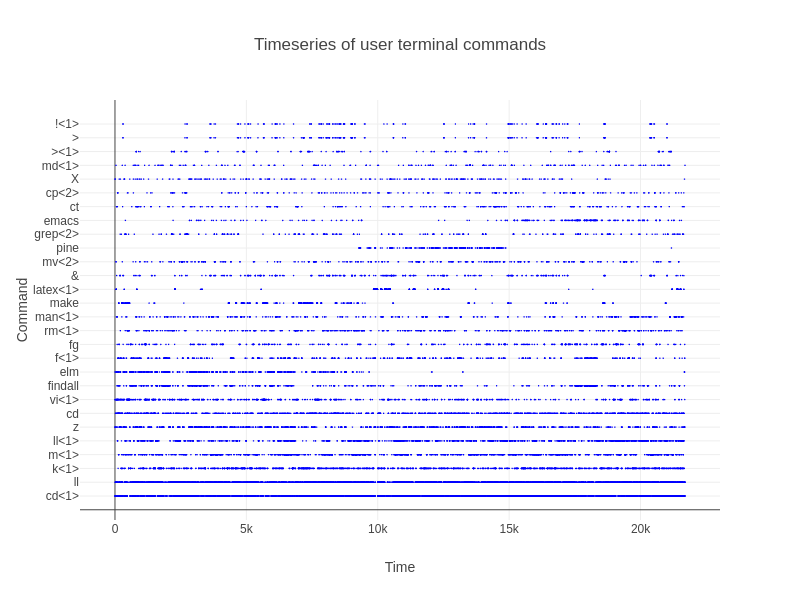
\includegraphics[scale=.45]{../pictures/complete-empirical-timeseries.png}
  \caption{Complete timeseries}
\end{figure}

\begin{figure}[!htb]
  \centering
  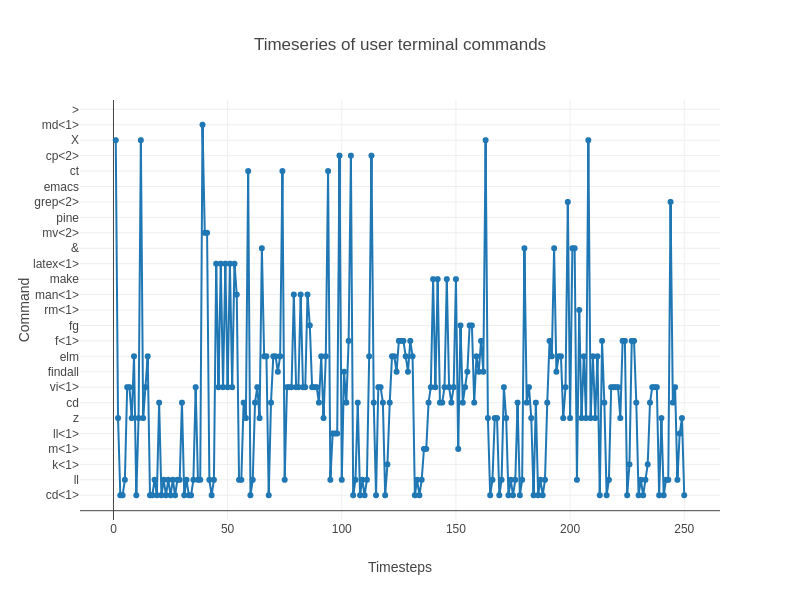
\includegraphics[scale=.45]{../pictures/250-empirical-timesteps.png}
  \caption{Shortened timeseries}
\end{figure}

We plotted the entire time series and the first 250 steps. (See page 2)

Note for the timeseries plot---on $250$ steps---how there are periods of time
where the chain alternates between two states. As an example, consider
\texttt{cd} and \texttt{ll}. As users of UNIX operating systems ourselves, this
is very common because \texttt{cd} is used to navigate through the computer's
file system and \texttt{ll} is used to view the files in a directory. As another
example, switching between \texttt{vi}, i.e. text editing, and \texttt{latex}
or \texttt{make} (which builds code) is also a common occurrence. This gave us
faith that we had properly cleaned and plotted the data.

\begin{figure}[!htb]
  \centering
  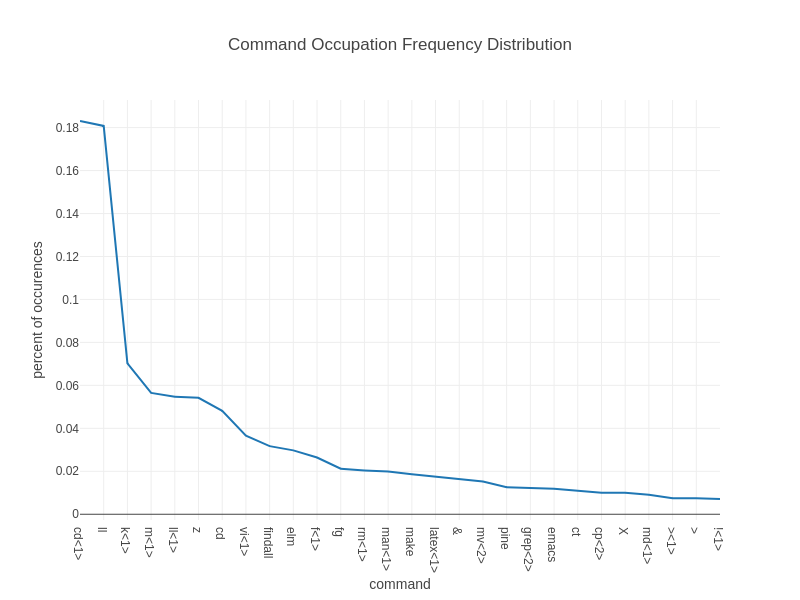
\includegraphics[scale=.50]{../pictures/empirical-occ-freq-dist.png}
  \caption{Occupation frequencies}
\end{figure}
\newpage
\section{Analysis}

We calculated the occupation frequencies of the empirical data by counting the
number of times each state was visited and graphed the distribution. (See Figure
$3$) Once again, as UNIX based operating system users ourselves, the
distribution seemed quite similar to our own experiences.

\begin{figure}[!htb]
  \centering
  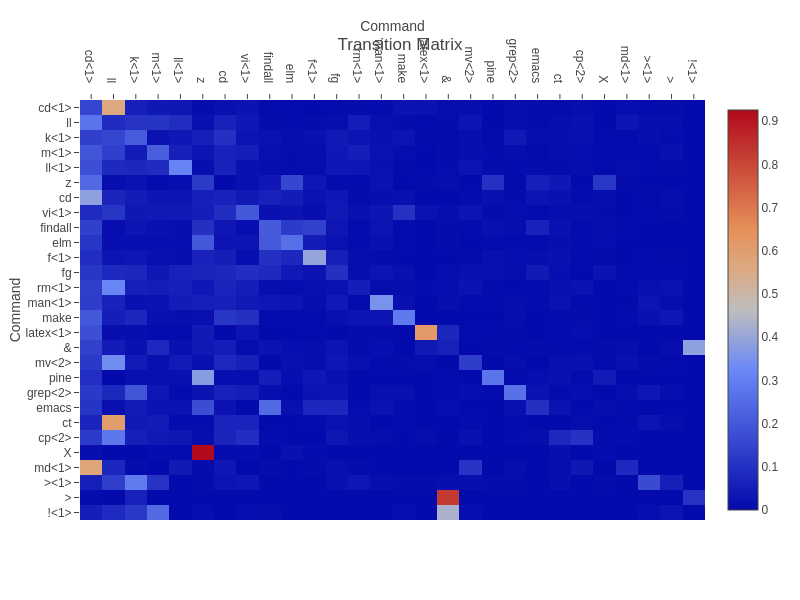
\includegraphics[scale=.50]{../pictures/transition-matrix-heatmap.png}
  \caption{The transition matrix}
\end{figure}

Next we computed the transition matrix by counting the number of times the chain
went from state $i$ to state $j$ followed by dividing each count $P_{ij}$ by the
number of times we moved out of state $i$. We plotted the transition matrix as a
heatmap (see Figure $4$), as we believe that this provides a much better
understanding of the transitions of the chain. 

Note the high(er) probabilities on the diagonal; after typing a command, you are
more likely to type it again than typing most others. Additionally, the column
for \texttt{cd<1>} is brighter than most; after every command you are decently
likely to navigate to another directory. 

We raised the transition matrix to the power $1000$ to compute the stationary
distribution. We argue that the original chain is irreducible because the data
tracks the user's usage of the UNIX machine over two years. This means that
there are many instances of logging in and out of the machine, which is done
with the same set of commands every time (\texttt{rlogin} and \texttt{exit}). So
the only instance where a state $i$ is unreachable from $j$ is if the user types
a command and then doesn't proceed to logoff or doesn't proceed to log on.

Both cases are impossible because a command isn't tracked until the user has
logged on and since we're tracking the $28$ most common commands there is no way
that one of these commands are used so frequently in conjunction with the user
never exiting afterwords.  Therefore, since the chain always visits the state
\texttt{exit} every other state can reach \texttt{exit} which means every  state
can reach every other state via the \texttt{exit} state.

Therefore our stationary distribution is unique and it is equal to a row of the
transition matrix raised to a high power. We plot the distribution against the
occupation frequency there is no surprise that the distributions are identical.
(See Figure $7$ in the Appendix) Since there are no zero values in the
stationary distribution and there are states that can loop back into themselves, the chain is regular.

\begin{figure}[!htb]
  \centering
  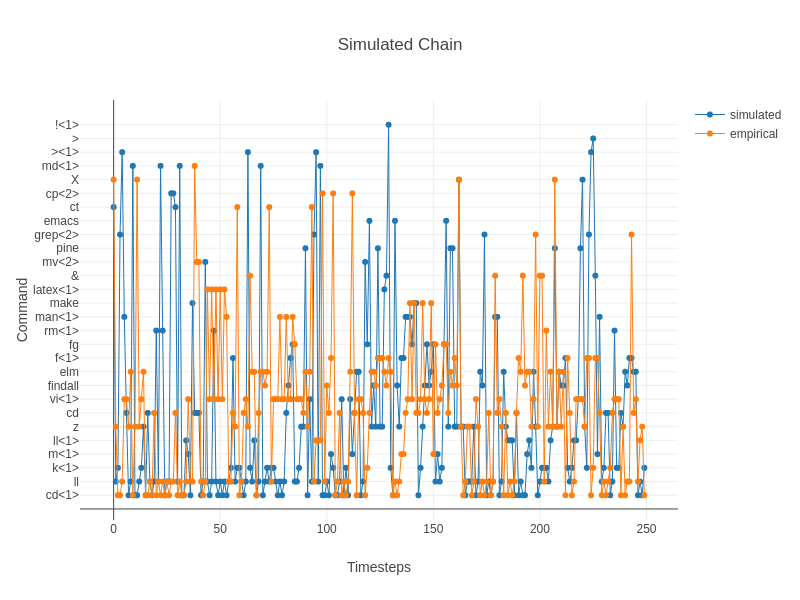
\includegraphics[scale=.45]{../pictures/simul-chain-vs-empirical-chain.png}
  \caption{Simulation timeseries}
\end{figure}

We simulated the chain for $250$ time steps. The initial state was chosen
uniformly at random over all the states. We plotted the simulation against the
empirical data. (See Figure 5)

The original chain has many back and forths between lesser (i.e. not \texttt{cd}
and \texttt{ll}) states, as discussed earlier, while the simulated chain does
not appear to capture this behavior. In general, the simulated chain appears to
lose much of the structure of the original chain, bobbing around meaninglessly
between states while the original chain has reoccurring patterns (though still
with meaningless jumps up to less used states).

Finally we investigated the mixing time of the chain. We did this by, at each
time step, computing the occupation frequency of the chain from the first to the
current time step. At each step we calculate the occupational frequency of the
states seen so far and subtracted this distribution with the calculated
stationary distribution. We then plotted the $L_1$ norm of the difference.

After $900$ steps it has a difference of around $0.1$, which is quite small. The
chain gets to a difference of $0.5$ after only $50$. The chain appears to
converge quite rapidly to the stationary distribution.

\begin{figure}[!htb]
  \centering
  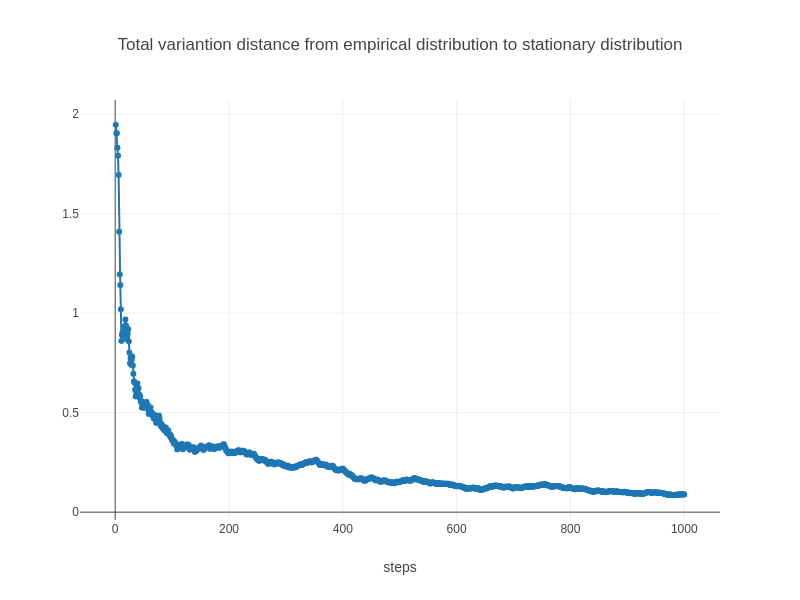
\includegraphics[scale=.45]{../pictures/mixing-time-analysis.png}
  \caption{Distance between true distribution and partial}
\end{figure}

\clearpage

\section{Appendix}

\begin{figure}[!htb]
  \centering
  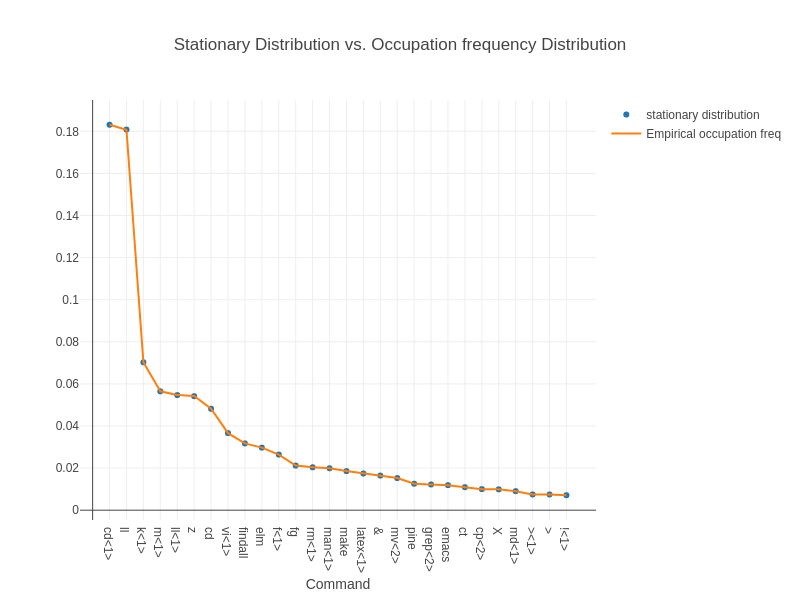
\includegraphics[scale=.50]{../pictures/stat-dist-and-empirical-occ-freq-dist.png}
  \caption{The calculated stationary distribution and the one derived from the data}
\end{figure}

\end{document}

